\documentclass{beamer}
%\usetheme{Boadilla}
\usetheme{default}

\usepackage{epstopdf}
\usepackage{listings}
\usepackage{subcaption}
\usepackage[utf8]{inputenc}
%\usepackage{unicode-math}
\usepackage{alltt}
\usepackage{booktabs}
\usepackage{fancyvrb}
\usepackage{multicol}

% In descriptions, start new line after label
\usepackage{enumitem}
\setlist[description]{style=nextline}

\newcommand{\tuple}[1]{\langle #1 \rangle}

\title{Arrp}
\subtitle{The Programming Language }
\author{Jakob Leben}
\institute{University of Victoria\\Department of Computer Science}
\date{Lyon, December 14, 2019}

\begin{document}

\begin{frame}
\titlepage
\end{frame}

\begin{frame}
\frametitle{Outline}
\tableofcontents
\end{frame}

\section{Motivation}

\begin{frame}[fragile]
\frametitle{Motivation - Language Design}

Variations of max filter:
% FIXME: Make figure instead
{
\footnotesize
\begin{align}
\label{eq:max-filter}
    y[n] &= \max_{i = 0}^{N-1} \; x[n+i] \\
    y[n] &= \max_{i = 0}^{N-1} \; x[Hn+i] \\
    y[n, j] &= \max_{i = 0}^{N-1} \; x[n+i, j], \quad 0 \leq j < M \\
    y[n] &= \max_{j = 0}^{M-1} \; x[n, j]
\end{align}
}

\vspace{-3em}
\begin{figure}
\begin{subfigure}[t]{0.4\textwidth}
    \caption{Composition}
    % NOTE: Save the SVG figures as PDF before building slides
    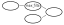
\includegraphics[width=\textwidth]{../build/stream_graph}
\end{subfigure}
\hspace{0.5cm}
\begin{subfigure}[t]{0.4\textwidth}
\caption{Implementation}
\footnotesize
\vspace{-1em}
\begin{verbatim}
class max_filter
{
max_filter(int N, int H, int dim)
{...}
void process(const float * x,
                   float * y)
{...}
}
\end{verbatim}
\end{subfigure}

\end{figure}

\end{frame}


\begin{frame}[fragile]
\frametitle{Motivation - Performance}

\[y[n, j] = \max_{i = 0}^{N-1} \; x[n+i, j], \quad 0 \leq j < M\]

\centering
\includegraphics[height=2.5in]{../build/parallel-scaling-max-filter-slide}

\end{frame}


\begin{frame}
\frametitle{Arrp}

\begin{itemize}
\item Design a language for stream processing that:
\begin{itemize}
  \item Allows straightforward translation from mathematical equations.
  \item Maximizes code reuse via modularity and abstraction.
\end{itemize}
\item Utilize the polyhedral framework to:
\begin{itemize}
  \item Avoid performance penalties of modularity and abstraction.
  \item Potentially compete with hand-written C.
\end{itemize}
\end{itemize}

\end{frame}

\section{The Arrp Language for Stream Processing}

\begin{frame}[fragile]
\frametitle{Familiar syntax}

\textbf{One-pole filter}
\[y[n] = b x[n] - a y[n-1]\]
\begin{center}
\begin{BVerbatim}
y[n] = b*x[n] - a*y[n-1];
\end{BVerbatim}
\end{center}

\textbf{FIR filter}
\[y[n] = \sum_{i = 0}^{N-1} \; b[i] x[n-i]\]
\begin{center}
\begin{BVerbatim}
y[n] = sum([i:N] -> b[i] * x[n-i])
\end{BVerbatim}
\end{center}

\textbf{Max filter}
\[y[n] = \max_{i = 0}^{N-1} \; x[n+i]\]
\begin{center}
\begin{BVerbatim}
y[n] = max_elem([i:N] -> x[n+i]);
\end{BVerbatim}
\end{center}

\end{frame}


\begin{frame}[fragile]
\frametitle{Polymorphic, higher-order functions}

\begin{center}
\begin{BVerbatim}
max_filter(N,x) = y where
    y[n] = max_elem([i:N] -> x[n+i]);

max_elem = fold((a,b) -> max(a,b));

fold(f,x) = r[#x-1] where {
    r[0] = x[0];
    r[i] = f(r[i-1], x[i]), if i < #x;
}
\end{BVerbatim}
\end{center}

\end{frame}



\begin{frame}[fragile]
\frametitle{Point-wise Operations, Multi-dimensional Streams}

\begin{center}
\begin{BVerbatim}
max_filter(N,x) = y where
    y[n] = max_elem([i:N] -> x[n+i]);

input x1 : [~]real32;
y1 = max_filter(10, x1);

input x2 : [~,10]real32;
y2 = max_filter(15, x2);
\end{BVerbatim}
\end{center}

\end{frame}


\begin{frame}[fragile]
\frametitle{Multi-rate Programs}

\begin{center}
\begin{BVerbatim}
downsample(x, factor) = [n] -> x[factor * n];

upsample(x, factor) = y where
    y[n] = {
        x[n / factor], if n % factor == 0;
        0,             otherwise
    };

max_filter(N, hop, x) = y where
    y[n] = max_elem([i:N] -> x[hop * n + i]);
\end{BVerbatim}
\end{center}

\end{frame}


\begin{frame}[fragile]
\frametitle{Physical Modeling}

\textbf{2d Wave Equation - FDTD\footnotemark}
\begin{center}
\begin{BVerbatim}
u[n,i,j] =
      b0 * u[n-2, i, j]
    + b1 * u[n-1, i, j]
    + b2 * (  u[n-1, i+1, j] + u[n-1, i, j+1]
            + u[n-1, i-1, j] + u[n-1, i, j-1] );
\end{BVerbatim}
\end{center}

\footnotetext{Stefan Bilbao. Numerical Sound Synthesis:
Finite Difference Schemes and Simulation in Musical Acoustics. 2009.}
\end{frame}



\begin{frame}[fragile]
\frametitle{Generated C++}

\footnotesize

\begin{minipage}{0.49\linewidth}
\begin{BVerbatim}
template <typename IO>
class program
{
public:
  IO * io;
  void prelude();
  void period();
private:
  double a;
  double y;
  double b;
};
\end{BVerbatim}
\end{minipage}\hfill
\begin{minipage}{0.49\linewidth}
\begin{BVerbatim}
template <typename IO>
inline void program<IO>::prelude()
{
  double x;
  io->input_b(b);
  io->input_a(a);
  y=0;
  io->input_x(x);
  io->output_y(y);
}

template <typename IO>
inline void program<IO>::period()
{
  double x;
  io->input_x(x);
  y=b*x-a*y;
  io->output_y(y);
}
\end{BVerbatim}
\end{minipage}

\end{frame}


\begin{frame}
\frametitle{Arrp - Functional Language Features}

\begin{itemize}
\item bindings of names to expressions and functions
\item function applications (including partial)
\item lambda abstractions (anonymous functions)
\item higher-order functions (with other functions as parameters)
\item polymorphic functions, type inference
\end{itemize}

\end{frame}

\begin{frame}[fragile]
\frametitle{Arrp - Arrays and Streams}

\[(D \subset \mathbb{Z}^d) \to V\]

Hyperrectangular index domain with one \textbf{infinite dimension}.
\vspace{\baselineskip}

Inline syntax (lambda abstraction, array comprehension):

\begin{semiverbatim}
y = [~,5: t,i -> x[t] * i];
\end{semiverbatim}

Alternative syntax (in development):

\begin{verbatim}
y[t,i] = x[t] * i   for i < 5;
\end{verbatim}

\end{frame}

\begin{frame}[fragile]
\frametitle{Arrp - Example: Max Filter}

\begin{align*}
y[n] &= \max_{i = 0}^{N-1} \; x[Hn+i]
\end{align*}

Implementation applies to x with any number of dimensions:

\vspace{1em}
\begin{Verbatim}[numbers=left]
max_filter(N,H,x) = y where
    y[n] = max_([N: i -> x[H*n + i]]);

max_ = fold(\a,b -> max(a,b));

fold(f,x) = r[#x-1] where {
    r[0] = x[0];
    r[i] = f(r[i-1], x[i])   for 0 < i < #x;
}
\end{Verbatim}

\end{frame}

\begin{frame}[fragile]
\frametitle{Reduction of Arrp to Recurrence Equations}

From this:

\begin{Verbatim}[numbers=left]
input x :: [~,20]real64;
main = max_filter(10,5,x);
\end{Verbatim}

To this:

\begin{Verbatim}[numbers=left]
x[n,j] = input(n,j)   for j < 20;
main[n,j] = r[n,9,j]  for j < 20;
r[n,0,j] = x[5*n, j]  for j < 20;
r[n,i,j] =  max(r[n,i-1,j], x[5*n+i, j])
                for 0 < i < 10 and j < 20;
\end{Verbatim}

\end{frame}

% FIXME: Maybe skip this slide - talk about this in conclusions/limitations/future work
%\begin{frame}
%\frametitle{Restrictions to affine expressions}
%\end{frame}

\section{Polyhedral Compilation of Streaming Programs}

\begin{frame}
\frametitle{Polyhedral Compilation - Overview}

(\textbf{Major contribution}, \textit{Minor contribution})

\begin{itemize}
\item \textit{Derive polyhedral model from source}
\item Find good schedule
    \begin{itemize}
    \item Affine schedule function
    \item Tiling for performance
    \item \textbf{Periodic Tiling}
    \item Choose parallel schedule dimensions
    \end{itemize}
\item \textit{Allocate memory}.
\item Generate C++ code
    \begin{itemize}
    \item \textbf{Extract prologue and period schedule}
    \item \textit{Generate code to execute schedule}
    \item \textbf{Generate stream buffer code}
    \item OpenMP annotation
    \end{itemize}
\end{itemize}


\end{frame}

\begin{frame}[fragile]
\frametitle{Periodic Tiling - Purpose}
{
\scriptsize
\begin{align}
x(n,i) &= \text{input}(n,i), \quad &0 \leq i < N\\
y(m,i) &= x(2m, i) + x(2m+1, i),  \quad &0 \leq i < N
\end{align}
}
\vspace{-2em}
\begin{figure}
    \begin{subfigure}[t]{0.32\textwidth}
        \includegraphics[width=\textwidth]{../build/downsample-sched-simple1}
        \caption{Unproductive}
        \label{fig:downsample-sched-pluto}
    \end{subfigure}
    \begin{subfigure}[t]{0.32\textwidth}
        \includegraphics[width=\textwidth]{../build/downsample-sched-simple2}
        \caption{Simple productive}
        \label{fig:downsample-sched-feasible}
    \end{subfigure}
    \begin{subfigure}[t]{0.32\textwidth}
        \includegraphics[width=\textwidth]{../build/downsample-sched-tiled}
        \caption{Periodically tiled}
        \label{fig:downsample-sched-periodic}
    \end{subfigure}

    \scriptsize
    \begin{subfigure}[b]{0.32\linewidth}
    \begin{alltt}
for c2 in 0..N:
  for c1 in 0..\(\infty\):
    x[c1\%2,c2] =
      input(c2);
    if (c1-1)\%2 == 0:
      output(...)
    \end{alltt}
    \end{subfigure}
    \begin{subfigure}[b]{0.32\linewidth}
    \begin{alltt}
for c1 in 0..\(\infty\):
  for c2 in 0..N:
    x[c1\%2,c2] =
      input(c2);
    if (c1-1)\%2 == 0:
      output(...)
    \end{alltt}
    \end{subfigure}
    \begin{subfigure}[b]{0.32\linewidth}
    \begin{alltt}
forever:
  for c2 in 0..N :
    x[0] = input(c2);
    x[1] = input(c2);
    output(x[0] + x[1]);
    \end{alltt}
    \end{subfigure}
\end{figure}

\end{frame}


\begin{frame}
\frametitle{Periodic Schedule Tiling}

\begin{itemize}
\item Minimal requirements for polyhedral model and schedule
\item A tiling with conditions for direction, offset, size w.r.t ray and vertices.
\item Algorithm:
\begin{itemize}
\item Find periodic tiling of individual array access schedules.
\item Compute maximum of the offsets.
\item Compute common multiple of the sizes.
\end{itemize}
\end{itemize}

\vspace{-1em}
\begin{figure}
\centering
\includegraphics[width=\textwidth]{../build/stencil-basic}
\caption{Two schedule dimensions. Bold dots highlight different statements.
Prologue: red. Periods: blue.}
\end{figure}

\end{frame}

\begin{frame}
\frametitle{Periodic Tiling and Performance Concerns}

\begin{figure}
\caption{Statement iterations. Dashed lines: \textbf{tile boundaries}. Red: \textbf{prologue}. Blue: \textbf{period}. Bold line: \textbf{parallelizable tiles}. Arrows: \textbf{dependencies}. Bottom dots: \textbf{input}. Top dots: \textbf{output}}
\centering
    \begin{subfigure}[t]{.22\linewidth}
    \includegraphics[height=1.3in]{../build/stencil-tiled0}
    %\captionsetup{skip=2pt}
    \caption{No parallelism}
    \label{fig:stencil-tiled1}
    \end{subfigure}
    \begin{subfigure}[t]{.26\linewidth}
    \includegraphics[height=1.3in]{../build/stencil-tiled1}
    %\captionsetup{skip=2pt}
    \caption{Large parallelism,\\Large latency}
    \label{fig:stencil-tiled2}
    \end{subfigure}
    \begin{subfigure}[t]{.26\linewidth}
    \includegraphics[height=1.3in]{../build/stencil-tiled2}
    %\captionsetup{skip=2pt}
    \caption{Balanced parallelism and latency}
    \label{fig:stencil-tiled3}
    \end{subfigure}
    \begin{subfigure}[t]{.22\linewidth}
    \includegraphics[height=1.3in]{../build/stencil-tiled3}
    %\captionsetup{skip=2pt}
    \caption{Large parallelism,\\No latency}
    \label{fig:stencil-tiled4}
    \end{subfigure}
\label{fig:periodic-and-classic-tiling}
\end{figure}

\end{frame}

\begin{frame}[fragile]
\frametitle{Storage Allocation and Code Generation}


Storage allocation: $\vec{i} \mapsto \vec{i} \bmod \vec{e}$.

\[y[n] = \max_{i = 0}^{N-1} \; x[n+i]\]

\vspace{-1em}
\begin{figure}
\footnotesize
\begin{subfigure}[t]{.45\linewidth}
\captionsetup{skip=0pt}
\caption{Traditional}
\begin{alltt}
x = new int[e]
// Initialize x[0..N-1]
for n in 0..\(\infty\)
  x[(n+N-1)\%e] = input()
  y = x[n\%e]
  for i in 1..N:
    y = max(y, x[(n+i)\%e])
  output(y)
\end{alltt}
\end{subfigure}
\begin{subfigure}[t]{.45\linewidth}
\captionsetup{skip=0pt}
\caption{Periodic (1 output / period)}
\begin{alltt}
x = new int[e]
d = 0
// Prologue: Initialize x[0..N-1]
forever:
  // Period:
      x[(d+N-1)\%e] = input()
      y = x[d\%e]
      for i in 1..N:
        y = max(y, x[(d+i)\%e])
      output(y)
  d = (d+1)\%e
\end{alltt}
\end{subfigure}

\end{figure}

\end{frame}




\section{Experiments}

\begin{frame}
\frametitle{Experiment 1}

Claim: Arrp provides convenience and modularity without performance penalty

\begin{table}
\centering
\begin{tabular}{c c c c c}
\hline
Application & Cycles & Speed & Buffers & Lines of Code \\
\hline
Synth & 0.37 & 2.70  & 1.58 & 0.24 \\
EQ & 1.09 & 0.92 & 1.03 & 0.14 \\
AC & 0.61 & 1.64 & 1.00 & 0.23 \\
\hline
Mean & \textbf{0.69} & \textbf{1.75} & \textbf{1.20} & \textbf{0.20}\\
\hline
\end{tabular}
\caption{Results of evaluation: Arrp / C++}
\label{tab.eval-results}
\end{table}

\end{frame}


\begin{frame}
\frametitle{Experiment 2}

Claim: Proposed polyhedral compilation of streaming programs enables data locality optimizations

\begin{figure}
\centering
\includegraphics[width=0.85\textwidth]{../build/parallel-scaling-slide}
\end{figure}

\end{frame}



\section{Conclusions and Future Work}

\begin{frame}
\frametitle{Conclusions}

\begin{itemize}
\item The language Arrp can enable more code reuse in some stream processing applications.
\item The polyhedral compilation technique:
  \begin{itemize}
  \item Reduces performance penalty of Arrp
  \item Could enable new optimizations for stream processing in general.
  \end{itemize}
\end{itemize}

\end{frame}

\begin{frame}
\frametitle{Future Work}

\begin{itemize}
  \item Language improvements
      \begin{itemize}
      \item Product types ("structs")
      \item Functional recursion
      \item Data-dependent and non-affine index bounds
      \end{itemize}
  \item Automatically optimize periodic tiling parameters to maximize throughput and minimize latency
  \item Combine with dataflow scheduling techniques for
      \begin{itemize}
      \item Task and pipeline parallelism
      \item Dynamic behaviors
      \end{itemize}
  \item Support alternative hardware:
      \begin{itemize}
      \item Heterogeneous (including GPU and other accelerators)
      \item Reconfigurable (FPGA)
      \item Application-specific hardware synthesis
      \end{itemize}
\end{itemize}

\end{frame}

\begin{frame}

\centering

Jakob Leben, Ph.D. candidate, University of Victoria
jakob.leben@gmail.com

\vspace{3em}
Arrp website: arrp-lang.info
\end{frame}

\begin{frame}
\frametitle{My Background}

\begin{itemize}

\item Bachelor of Arts in Philosophy
    \begin{itemize}
    \item University of Ljubljana, Slovenia, 2010.
    \item Thesis Topic: Aesthetics of computer generated art.
    \end{itemize}

\item Master's Degree in Sonology
    \begin{itemize}
    \item Institute of Sonology, Royal Conservatoire, The Hague, The Netherlands, 2012.
    \item Thesis Topic: Algorithms in musical performance.
    \end{itemize}

\item Project: SuperCollider Development

\item Project: Automatic Segmentation of Ethnomusicological Audio Recordings

\end{itemize}

\end{frame}

\begin{frame}
\frametitle{Motivation - Language Design}

FDTD for 2d wave equation:

\begin{equation}
\label{eq:wave-2d}
\begin{aligned}
u[n,i,j]
    &= b_0 u[n-2,i,j] + b_1 u[n-1,i,j] \\
    &+ b_2 \big(u[n-1,i-1,j] + u[n-1,i+1,j] \\
    &+ u[n-1,i,j-1] + u[n-1,i,j+1]\big), \\
    &0 < i < M-1, \quad 0 < j < N-1\\
\end{aligned}
\end{equation}

Hard to express in any other way.

\end{frame}


\begin{frame}
\frametitle{Motivation - Performance}

Spectrum flux:

\begin{equation}
\label{eq:flux}
y[n] = \sum_{i = 0}^{N} x[n, i] - x[n-1, i]
\end{equation}

Separate difference and summation:
\begin{align}
\label{eq:flux}
w[n,i] &= x[n, i] - x[n-1, i], \quad 0 \leq i < N\\
y[n] &= \sum_{i = 0}^{N} w[n, i]
\end{align}

More modular, but large overhead of intermediate array w.

\end{frame}


\begin{frame}[fragile]
\frametitle{Arrp - Multi-rate Signal Processing}

\begin{verbatim}
downsample(x, factor) = [n -> x[n * factor]];

repeat(x, factor) = [n -> x[n / factor]];

upsample(x, factor) = y where {
    y[n] = x[n / factor]  for n % factor == 0;
    y[n] = 0;
}
\end{verbatim}

\end{frame}


\begin{frame}
\frametitle{Periodic Tiling in Abstract}

\[\tau(\vec{i}) = \lfloor(\vec{d} \cdot \vec{i} - \mu)/\sigma\rfloor, \quad \text{where}\]

\begin{center}
\begin{tabular}{c c c}
(1) $\; \vec{d} \cdot \vec{r} > 0 \quad$ &
(2) $\; \mu \geq \max \,\{ \vec{d} \cdot \vec{v} \;|\; \vec{v} \in V \} \quad$ &
(3) $\; \sigma = \vec{d} \cdot \vec{r}$
\end{tabular}
\end{center}

\begin{figure}
  \begin{subfigure}[t]{.32\linewidth}
    \includegraphics[width=\textwidth]{../build/periodic-tiling}
    \caption{$\vec{d} = \tuple{1,0}$, $\mu = 4$, $\sigma = 2$.
        %The smallest ray of the polyhedron is $\vec{r} = \tuple{2,1}$.
        %Prologue tiles are red and periodic tiles blue.
    }
    \label{fig:periodic-tiling:a}
  \end{subfigure}
  \begin{subfigure}[t]{.32\linewidth}
    \includegraphics[width=\textwidth]{../build/tiling-wrong-size}
    \caption{$\vec{d} = \tuple{1,0}$, $\mu = 3$, $\sigma = 3$.
        %is not a periodic tiling:
        %$\sigma$ is not an integer multiple of $\vec{d} \cdot \vec{r}$
    }
    \label{fig:periodic-tiling:b}
  \end{subfigure}
  \begin{subfigure}[t]{.32\linewidth}
    \includegraphics[width=\textwidth]{../build/tiling-wrong-direction}
    \caption{$\vec{d} = \tuple{-1,2}$, $\mu = 4$, $\sigma = 2$.
        %is not a periodic tiling:
        %$\sigma$ is not an integer multiple of $\vec{d} \cdot \vec{r}$
    }
    \label{fig:periodic-tiling:c}
  \end{subfigure}
  \caption{A periodic tiling (a), and two non-periodic tilings (b and c).}
  \label{fig:periodic-tiling}
\end{figure}

\end{frame}


\begin{frame}
\frametitle{Periodic Tiling in Abstract}

Periodic tiling $\tuple{\vec{d}, \mu, \sigma}$: $\tau(\vec{i}) = \lfloor(\vec{d} \cdot \vec{i} - \mu)/\sigma\rfloor$

\vspace{-1em}
\begin{figure}
  \caption{A periodic tiling (a), and two non-periodic tilings (b and c).}
  \begin{subfigure}[t]{.32\linewidth}
    \includegraphics[width=\textwidth]{../build/periodic-tiling}
    \caption{$\vec{d} = \tuple{1,0}$, $\mu = 4$, $\sigma = 2$.
        %The smallest ray of the polyhedron is $\vec{r} = \tuple{2,1}$.
        %Prologue tiles are red and periodic tiles blue.
    }
    \label{fig:periodic-tiling:a}
  \end{subfigure}
  \begin{subfigure}[t]{.32\linewidth}
    \includegraphics[width=\textwidth]{../build/tiling-wrong-size}
    \caption{$\vec{d} = \tuple{1,0}$, $\mu = 3$, $\sigma = 3$.
        %is not a periodic tiling:
        %$\sigma$ is not an integer multiple of $\vec{d} \cdot \vec{r}$
    }
    \label{fig:periodic-tiling:b}
  \end{subfigure}
  \begin{subfigure}[t]{.32\linewidth}
    \includegraphics[width=\textwidth]{../build/tiling-wrong-direction}
    \caption{$\vec{d} = \tuple{-1,2}$, $\mu = 4$, $\sigma = 2$.
        %is not a periodic tiling:
        %$\sigma$ is not an integer multiple of $\vec{d} \cdot \vec{r}$
    }
    \label{fig:periodic-tiling:c}
  \end{subfigure}
\end{figure}

\vspace{-2em}
\begin{itemize}
\item Each tile $\tau(\vec{i}) \geq 0$ has a finite number of points.
\item $\tau(\vec{i}) + 1 = \tau(\vec{i} + \vec{r})$
\end{itemize}

\end{frame}

\begin{frame}
\frametitle{Periodic Schedule Tiling}
\scriptsize
\[0 \leq n, \quad 0 \leq m, \quad 0 < i < N-1, \quad K = \lfloor N/2 \rfloor\]
\begin{align}
&s_1: x(n) = \text{input}(n) \\
&s_2: u(n,0) = u(n,N-1) = 0 \\
&s_3: u(0,i) = x(0) \\
&s_4: u(n,i) = x(n) + u(n-1,i) + u(n-1,i-1) + u(n-1,i+1)\\
&s_5: y(m) \gets u(2m, K)
\end{align}

\begin{figure}
\centering
\includegraphics[width=\textwidth]{../build/stencil-basic}
\caption{Two schedule dimensions. Highlighted statements (left to right): $s_1$, $s_2$, $s_3$, $s_4$, $s_5$.
Prologue: red. Periods: blue.}
\end{figure}

\end{frame}


\begin{frame}
\frametitle{Storage Allocation}

\begin{definition}[Modular mapping $\tuple{M, \vec{e}}$]
Store array element $\vec{i}$ into location $M \vec{i} \bmod \vec{e}$.
\end{definition}

\begin{theorem}
The successive modulo technique (SM)\footnotemark yields a modular mapping $\tuple{M, \vec{e}}$ with a \textbf{finite} storage size $\vec{e}$ for any
\textbf{periodically tiled} rate-consistent schedule and any $M$.
\end{theorem}

\footnotetext{Vincent Lefebvre and Paul Feautrier. Automatic storage management for parallel
programs. Parallel Computing, 24(3-4), 1998.}

\end{frame}


\begin{frame}[fragile]
\frametitle{Buffer Optimization}

\begin{figure}
\footnotesize
\begin{subfigure}[t]{.45\linewidth}
\caption{Bitmask instead of modulo}
\begin{alltt}
E = next_power_of_two(e)
M = E-1 // e.g. 100 -> 011
x = new int[E]
d = 0
// Initialize x[0..N-1]
forever:
  x[(d+N-1)&M] = input()
  y = x[d&M]
  for i in 1..N:
    y = max(y, x[(d+i)&M])
  output(y)
  d = (d+1)&M
\end{alltt}
\end{subfigure}
\begin{subfigure}[t]{.45\linewidth}
\caption{Data shifting}
\begin{alltt}
E = 3*N
x = new int[E]
d = 0
// Initialize x[0..N-1]
forever:
  x[d+N-1] = input()
  y = x[d]
  for i in 1..N:
    y = max(y, x[d+i])
  output(y)
  d = (d+1)
  if d+N-1 == E:
    copy(x,0,E-N,N)
    d = 0
\end{alltt}
\end{subfigure}

\end{figure}

\end{frame}



\begin{frame}
\frametitle{Experiment 2 - Storage Size and Latency}

\scriptsize

\begin{table}
  \centering
  \input{../build/buf-mode-storage}
  \caption{Storage size in Mb for different implementations and buffer types.}
  \label{table:buf-mode-storage-size}
\end{table}

\vspace{-20pt}
\begin{table}
\centering
\begin{tabular}{l c c c c c}
\toprule
Algorithm & \multicolumn{2}{c}{C++ AO/HO} & \multicolumn{2}{c}{Arrp} \\
\midrule
filter-bank & $O(1)$ & 0 & $O(T)$ & 127 \\
max-filter  & $O(1)$ & 0 & $O(T)$ & 255 \\
ac          & $O(1)$ & 1 & $O(1)$ & 0 \\
wave1d      & $O(1)$ & 0 & $O(PT) \cap O(N^2)$ & 1537 \\
wave2d      & $O(1)$ & 0 & $O(PT) \cap O(N)$ & 550 \\
\bottomrule
\end{tabular}
\caption{Logical latency (complexity and value). $N$ is algorithm scale (2000), $T$ is tile size (32-500), $P$ is degree of parallelism (6).}
\label{table:latency}
\end{table}

\end{frame}


\end{document}

